\documentclass[10pt,a4paper]{article}
\usepackage{multirow}
\usepackage{bm}
\usepackage{amsfonts}
\usepackage{amssymb}
\usepackage{amsmath} 
\usepackage{latexsym}
\usepackage{graphicx}
\usepackage{subfigure}
\usepackage{authblk}
\usepackage{listings}
\usepackage[T1]{fontenc}
\usepackage[colorlinks,linkcolor=blue]{hyperref}
\textwidth 6.5in
\textheight 8in
\topmargin 0pt
\linespread{1.5}
\oddsidemargin 0pt
\title{\huge STA237 Proje}
\newtheorem{coro}{\hskip 2em Corollary}[section]
\newtheorem{remark}[coro]{\hskip 2em Remark}
\newtheorem{propo}[coro]{\hskip 2em  Proposition}
\newtheorem{lemma}[coro]{\hskip 2em Lemma}
\newtheorem{theor}[coro]{\hskip 2em Theorem}
\newenvironment{prf}{\noindent { Proof:} }{\hfill $\Box$}
\date{6/8/2014}
\author[1]{Yilun Zhang \qquad  Xu Liu\qquad Han He}
\begin{document}
\maketitle
\begin{center} Paper title: The detection and estimation of long memory in stochastic volatility.\end{center}

\begin{center} Author: F.Jay Breidt, Nuno Crato, Pedro de Lima.\end{center}

\section{Background introduction}

We know that capital markets always show characters of non-linearity,and long-term memory is the most important feature of non-linear systems.In fact, many economists believe that asset market is a non-linear system with many uncertainties. Many researches have shown that the conditional volatility of asset prices show long memory or long-range persistence.(ie Although an asset return series has no serial correlation,the ACF of the squared or absolute-valued series of the return always decays at a hyperbolic rate as the lag increases.)We can see the BET stock index  \footnote[1]{The data and Rcode of this paper is downloadable from Yilun's github: \url{https://github.com/lunge111/STA237PROJECT}} as an example. The following plot is the sample ACF of daily returns for BET stock index from November 12,1999 to June 2,2014(Figure 1).

\begin{figure}[!htb]
\centering
\includegraphics[scale = 0.65]{return.png}
\caption{}
\end{figure}

Then we can compare it with the sample ACF of squared returns(Figure 2) and log squared returns as the following two plots(Figure 3).

\begin{figure}[!htb]
\centering
\includegraphics[scale = 0.65]{squaredreturn.png}
\caption{}
\end{figure}

\begin{figure}[!htb]
\centering
\includegraphics[scale = 0.65]{logsquared.png}
\caption{}
\end{figure}



In addition, we can also plot the log absolute returns for the same data to compare the patterns as the following(Figure 4).

\begin{figure}[!htb]
\centering
\includegraphics[scale = 0.65]{logabsreturn.png}
\caption{}
\end{figure}

Here we need to mention that BET is the reference index for the BVB,Bucharest Stock Exchange market.In BVB  there are traded shares,rights, bonds fund units and etc. BET is a free float weighted capitalization index of the most liquid 10 companies listed on the BVB regulated market.Thus this index methodology allows BET to be a powerful indication of the BVB market.Here we can clearly see the patterns we have mentioned before, the log squared or log absolute returns are decaying at a hyperbolic rate as the lag increases.

 In fact,traditional analyzing methods mainly focus on the short-term analysis,thus they cannot appropriately discribe the cases in the asset market, especially  the stochastic volatility  of asset prices.For a short memory process, its ACF or $\rho(h)$ willbe bounded at geometric rate, meaning that $|\rho(h)|\leq C r^{|h|}$ for some $C>0,\  0<r<1 $On the contrary,for a long memory process, its ACF decays as a hyperbolic rate, meaning that $\rho(h)\sim Ch^{2d-1}$ when $h$ increases to infinity.where $C\neq 0$ and $d<0.5$ In particular,when we focus on the long memory process with $0<d<0.5$,then we have $\sum |\rho(h)|=\infty$ we call this property persistent .
In order to test and estimate the persistent process, the paper we read gives a new method called long memory stochastic volatility(LMSV) model to represent the persistence in conditional variance and the authors have shown the superiority of the model when compared with many well known short-memory volatility models such as ARCH,GARCH,EGARCH and etc.




 
\section{Superiority of LMSV Model}

In the paper, the authors first listed the existing short-memory volatility models.

\vspace{0.5cm}

1. GARCH model 

\begin{center}$\displaystyle y_t=\sigma_t\epsilon_t$\end{center}

\begin{center} $\displaystyle \sigma_t^2=w+\sum_{j=1}^{q}b_j\sigma^2_{t-j}+\sum_{j=1}^{p}a_jy^2_{t-j} $ \end{center}

where $y_t$ is the prediction error (shock in the asset market ),$ \{ \epsilon_t\} $is independent and identically distributed with mean 0 and variance 1.$\sigma^2_t$ is the conditional variance of $y_t $given information at period t-1.
coefficients $\{a_j\}$ and $\{b_j\}$need to satisfy certain conditions.

In addition,we can rewrite it in the following form.

\begin{center}$\displaystyle b(B)\sigma^2_t=w+a(B)y^2_t$\end{center} 

where b(z)and a(z) are the autoregressive polynomial and moving average polynomial respectively.GARCH model is very popular in financial data because it can be used to discribe and predict the mean and variance of the return given the previous information, in practice, even a simple specifications in GARCH model has proven to be used successfully in predicting conditional variance,the volatility of returns. For example, in the foreign exchange markets, GARCH (1,1) could be a very power model in terms of the result of the predictions.

  But GARCH model is not a perfect model. In fact,it assumes that positive asset returns and negative asset returns have the symmetric effects,which is not always reasonable.For example, in the stock market,many observations have shown that the distribution of returns have fat tails,what is more, when there is a negative shock in the stock market, the stock price will go down usually, the volatility will also bocome greater in most cases. On the contrary, when there is a postive shock in the market, the stock price will go up, but usually the volatility will not become bigger and bigger,instead, it always stops increasing at some levels. Thus we need better model to discribe the asymmetry, EGARCH model is just one of the choices.

\vspace{0.5cm}

2. EGARCH model

 EGARCH model is very similar to the GARCH model.But it overcomes the weakness we mentioned above. 

\begin{center}$\displaystyle log\sigma^2_t=\mu_t+\sum_{j=0}^{\infty}\psi_j g(\epsilon_{t-j-1}) $\end{center}

Here the coefficients can be either positive or negative since $log(\sigma^2_t)$ can be negative here.Thus there will be no (fewer) restrictions on the parameters.$g(.)$ can be chosen, we may choose one as the following for example.
 
\begin{center}$\displaystyle g(\epsilon_t)=\theta\epsilon_t+r\{|\epsilon_t|-E(|\epsilon_t|)\}$\end{center} where $\theta$ and r are real constants.$\epsilon_t$ distributes with mean 0 and they are iid.$E(g(\epsilon_t))=0$,here we can see that $g(\epsilon)$ is asymmetric. 

Then we can also rewrite it in the following form.

\begin{center}$\displaystyle \phi(B)(log\sigma^2_t-\mu_t)=\theta(B)g(\epsilon_{t-j-1})$\end{center}

where $\phi(z)$\ and \ $\theta(z)$ are the autoregressive polynomial  and moving average polynomial respectively. As we have seen, EGARCH model is using the logarithm of the variance,but this may lead to a biased forecasts of variances, since by Jensen'inequality,$E(\sigma^2_t)\geq exp(E(log(\sigma^2_t)))$. What is more,similary with GARCH model, a simple EGARCH model is complex enough to discribe the volatility in practice in financial field.





From above, we now can see that both GARCH model and EGARCH model can be expressed in ARMA form,they are considered from the short-memory point of view,not the long memory model,thus the authors considered the following model.


  
  To introduce the next considered models, first, we introduce the long-memory process and ARFIMA model.\\
  
  For a discrete time series process $v_t$ with autocorrelation function $\rho (h)$ at lag h, the process is long-memory if the quantity
$$\lim\limits_{n\rightarrow\infty} \sum_{h=-n}^{n}|\rho(h)|$$
is nonfinite.Consequently,the spectral density $f(\omega)$ could be unbounded at low frequencies. However, a stationary and invertible ARMA process will always have a geometrically bounded autocorrelations and is a short memory process. Fractionally integrated process is a long memory process. For a simple case, consider the following,
$$(1-B)^dv_t=\eta_t$$
where B is the lag operator. When $-0.5<d<0.5$,and $\eta_t$ is a stationary process with a bounded valued spectrum at all frequencies. When $d=0$,the process is covariance stationary. When $0<d<0.5$,the process is long-memory and its autocorelations decay at a hyperbolic rate. When $-0.5<d<0$, the sum of absolute values of the autocorrelations tends to a constant.Thus, it is short memory.\\

 More generally, we can define an ARFIMA process,ARFIMA(p,d,q) model, as follows,
$$\phi(B)(1-B)^d(y_t-\mu)=\theta(B)\epsilon_t$$
where d is the fractional differencing parameter and $\epsilon_t$ is white noise. For $0<d<0.5$,the autocorrelation function,$\rho(.)$,is proportional to $k^{2d-1}$ as $k\rightarrow\infty$. Then, the autocorrelation of the ARFIMA process decay hyperbolically to zero as $k\rightarrow\infty$ which is different from geometric decay of a stationary ARMA process. Also for $0<d<0.5$, $\sum_{h=-n}^{h=n} |\rho(h)|$ diverges as $n\rightarrow \infty$,the process exhibits long memory. For $-0.5<d<0$, the process is said to exhibit intermeidiate memory.  \\

3. Long-memory GARCH and EGARCH model.\\

Given the weaknesses of the GARCH and EGARCH model in fitting this kind of data, the author introduces long memory models to solve the problem. The main motivation behind this is that although the dependence between distant observations is small, it is not negligible.\\
  To model such "long-term persistence", permitting the degree of differencing $d$ to be real values instead of integers is a good way as discussed above. Specifically from the above, when $0<d\leq 0.5$,the fractionally differenced processes show the property of long memory processes. Thus, it is reasonable to generalize GARCH models by using fractional differencing oprator defined through the expansion

\begin{center}$\displaystyle (1-B)^d=\sum_{j=0}^{\infty}\frac{\Gamma(j-d)}{\Gamma(j+1)\Gamma(-d)}B^j $\end{center}

Thus the fractionally integrated GARCH (FIGARCH) model is the following,

\begin{center}$\displaystyle (1-B)^db(B)(\sigma^2_t-\mu)=a(B)(y^2_t-\mu) $\end{center}
which means
$$\sigma^2=\mu+(1-B)^{-d}a(B)b^{-1}(B){y_t}^2=\mu+\sum_{j=1}^{n}\phi_j(y_{t-1-j}^2-\mu)$$
And avoiding the possibility of $\sigma_t^2<0$ leads to the situation where the use of spectral and time-domain autocorrelation methods is not justifiable in the standard way. Furthermore, problems occur when estimating the parameters.\\
Similar midifications can be applied to EGARCH models, we can obtain fractionally integrated EGARCH models. However, it is difficult to obtain good estimators in this model since asymtotic situation makes it hard to estimate the parameters.

\section{Long memory stochastic volatility (LMSV) model}
As we can see from above, both long-memory GARCH and EGARCH models are not appropriate in this case. Thus, the author consider the following long-memory stochastic volatility model. \\
First, we introduce the stochastic volatility model. 
In order to increase flexiblity of describing the evolution of $\sigma^2$,an alternative way is to add an innovation $v_t$ to the conditional variance equation of $y_t$.This is called a stochastic volatility.The model is defined by
$$y_t=\sigma_t\epsilon_t, \qquad \sigma_t=\sigma exp(v_t/2)$$
where {$\{v_t\}$} is independent of {$\{\epsilon_t\}$},{$\{\epsilon_t\}$} is independent and identically distributed with mean zero and variance one.
In our case, we need to fit a long memory data, thus, it is resonable to modify the model to long memory version by incorporating an ARFIMA process in a standard stochastic volatility model.Generally speaking,$\{v_t\}$ can be modeled as an ARFIMA(p,d,q),\cite{baillie1996long} defined as follows,
$$(1-B)^d\phi(B)v_t=\theta(B)\eta_t$$
where $\{\eta_t\} i.i.d N(0,\sigma_\eta^2)$ \\\\
The series can be analyzed as the following,
\begin{center}$\displaystyle log(y^2_t)=log(\sigma^2)+v_t+log(\epsilon^2_t)=\{log(\sigma^2)+E(log\epsilon^2_t)\}+v_t+\{log(\epsilon^2_t)-E(log(\epsilon^2_t))\}$\end{center}
\begin{center} $\displaystyle x_t=\mu+v_t+e_t$\end{center}
This is a long-memory Gaussian signal plus an i.i.d,non- Gaussian noise.This transformed series is easy to analyze.

Next,we will show the performance of long-memory test and emperical evidence. And it shows the superiority of model.
\section{Test for long memory}
In this part, we want to test whether a process is short 
 memory or long memory, ie, the $d$ in the model predefined is 0 or not. The paper provide two ways of test.
\subsection{Regression on frequency domain}

Let$u_t=(1-B)^dx_t$, $f_\beta(\lambda)^{(x)}$ is the spectral density of $x_t$ based on parameter $\bm{\beta} $, $f_\beta(\lambda)^{(u)}$ is the spectral density of $u_t$
$$f_\beta(\lambda)^{(x)}=\frac{\sigma_\eta^2|\theta(e^{-i\lambda})|^2}{2\pi|1-e^{-i\lambda}|^{2d}|\phi(e^{-i\lambda})|^2}+\frac{\sigma^2_\epsilon}{2\pi}=|1-e^{-i\lambda}|^{-2d}f_\beta(\lambda)^{(u)}+\frac{\sigma^2_\epsilon}{2\pi}$$
Taking logarithms in both sides 
\[
\log f_\beta(\lambda)^{(x)}=\log f_\beta(0)^{(u)}-d\log |1-e^{-i\lambda}|^{2}+\log\frac{f_\beta(\lambda)^{(u)}}{f_\beta(0)^{(u)}}+\log\frac{\sigma^2_\epsilon}{2\pi}\\
\] Replacing $\lambda$ by Fourier Sequency and adding $\log I_n(\omega_j)$ to both side.
\begin{eqnarray*}\log I_n(\omega_j)&=&\log f_\beta(0)^{(u)}-d\log |1-e^{-i\omega_j}|^{2}+\log\frac{f_\beta(\omega_j)^{(u)}}{f_\beta(0)^{(u)}}+\log\frac{\sigma^2_\epsilon}{2\pi}+\log\frac{ I_n(\omega_j)}{f_\beta(\omega_j)^{(x)}}\\
&=&\log f_\beta(0)^{(u)}+\log\frac{f_\beta(\omega_j)^{(u)}}{f_\beta(0)^{(u)}}+\log\frac{\sigma^2_\epsilon}{2\pi}+E(\log\frac{ I_n(\omega_j)}{f_\beta(\omega_j)^{(x)}})\\
&-&d\log |1-e^{-i\omega_j}|^{2}\\
&+&\log\frac{ I_n(\omega_j)}{f_\beta(\omega_j)^{(x)}}-E(\log\frac{ I_n(\omega_j)}{f_\beta(\omega_j)^{(x)}})
\end{eqnarray*}

When $\omega_j$ is close to 0, by continuity of $f_\beta(\omega_j)^{(u)}$, $\log\frac{f_\beta(\omega_j)^{(u)}}{f_\beta(0)^{(u)}}$ should be close to 0. We neglect it. 

let $y_i=\log I_n(\omega_j)$, $a=\log f_\beta(0)^{(u)}+\log\frac{f_\beta(\omega_j)^{(u)}}{f_\beta(0)^{(u)}}+\log\frac{\sigma^2_\epsilon}{2\pi}+E(\log\frac{ I_n(\omega_j)}{f_\beta(\omega_j)^{(x)}})$, $x_i=\log |1-e^{-i\omega_j}|^{2}$, $\epsilon_i=\log\frac{ I_n(\omega_j)}{f_\beta(\omega_j)^{(x)}}-E(\log\frac{ I_n(\omega_j)}{f_\beta(\omega_j)^{(x)}})$ ($I_n(\omega_j)=  f_\beta(\omega_j)^{(x)}\xi_j$, asymptotically , where $\xi\sim EXP(2\pi)$, $\epsilon_i's$ are identical uncorrelated mean 0 error). Fitting least square regression, $y_i=a+bx_i+\epsilon_i$, $d=-b$.

Do a usual t-test for the hypothesis $H_0: \, d=0$ to test whether it is long memory.

Because we assume $\omega_j$ close to 0, we are suggested to use first $n^u$ ordinates of peridogram. To avoid bias a additional first few truncation, $n^{0.1}$, should be done.

According to $\emph{Brockwell and Davis p530}$\cite{series1997springer}, $$\hat{d}\,is\,AN(d,\pi^2/\left[6\sum_{i=1}^{m}(x_i-\bar{X})\right])$$
When $d\in(-0.5,0)$

\subsection{R/S test}
Define ajdusted range $R$ as \[
R(n)=\max_{1\le k\le n}\left\{\sum_{i=1}^{k}X_i-\bar{X}\right\}-\min_{1\le k\le n}\left\{\sum_{i=1}^{k}X_i-\bar{X}\right\}
\]
Define normalization factor $S^2$ as \[
S^2(n,q)=\sum_{j=-q}^{j=q}w_q(j)\hat{\gamma}(j)
\] where $w_q(j)$ is the Bartlett window and q is given by 0 200 or \emph{data dependent formula $q^*=\lfloor (1.5n)^{1/3}(2\hat{\rho}(1)(1-\hat{\rho}^2(1))^{2/3}\rfloor$}
The $R/S$ statistics is $$Q(n,q)=\frac{R(n)}{S(n,q)}$$
Hust  exponent $J$ is estimated by $$\hat{J}(n,q)=\frac{\log Q(n,q)}{\log n}$$
 $\hat{J}(n,q)$ will weakly converge to 0.5 under short memory hypothesis, while it will converge to a constant larger than 0.5.

Suppose existence of $4+\delta$ moment $\delta>0$, under short memory hypothesis $V=n^{-1/2}Q(n,q)$ will weakly converge to a r.v has c.d.f $$F_V(v)=\sum_{k=-\infty}^{\infty}(1-4v^2k^2)e^{-2v^2k^2}$$ 

Even if a short memory process don't have finite second order moments, $\hat{J}(n,0)$ will converge to $\frac{1}{2}$. Hence it is still an indication of long memory.

\subsection{Simulation Study and Empirical evidence}
We use the model in section 4 to test long memory. We use arfima.sim() function in arfima package to generate simulations of ARFIMA(p,d,q) processes. We assume $\eta,\, \epsilon$ are standard Gaussian. Thus in each realization we generate sample size of 10000 ARFIMA(p,d,q) process with stand deviation 1 plus 10000 log $\chi^2(1)$ noise. We conduct both regression and R/S test on 100 replication and calculate mean, standard deviation and rejection proportion.

The spectral regression test is basic two-sided level 0.05 t-test. According to Lo(1991)\cite{lo1989long}, $V=Q(n,q)/\sqrt{n} \to \infty$ when $d\in(0.5,1)$, and $V=Q(n,q)/\sqrt{n} \to 0$ when $d \in (0,0.5)$. Therefore the test should be two sided, we conduct equal tail level 0.05 test. 
\begin{table}[!hbp]
\begin{tabular}{llllllll}
\hline
\hline
Model & $\hat{d}_{u=0.45}$ & $\hat{d}_{u=0.5}$ & $\hat{d}_{u=0.55}$ & $\hat{J}(n,0) $& $\hat{J}(n,q^*) $&$\hat{J}(n,200)$ \\
\hline
ARSV:$\phi=0.9,\,\sigma_\eta^2=0.45$ & 0.0132 & 0.0321 &  0.0731 & 0.6223 &     0.547 & 0.5230 \\
sd& 0.0931 & 0.0684  & 0.0541 & 0.0235  &   0.023 &  0.0205\\
Reject Proportion & 0.0200 &  0.0500  & 0.2400 & \,  &   0.180 & 0.0200\\
LMSV:$\d=0.47,\,\sigma_\eta^2=0.37$ & 0.3737 & 0.3551 &  0.3306 & 0.6983 &   0.6675 & 0.5719 \\
sd& 0.0976 & 0.0748  & 0.0532 & 0.0357 &   0.0312 & 0.0235\\
Reject Proportion & 0.9600 & 1.0000  & 1.0000 & \,  &  1.0000 & 0.6000\\
\hline
ARSV:$\phi=0.95,\,\sigma_\eta^2=0.23$ & 0.0571 &  0.123 &  0.2143 & 0.6518  &  0.5632 & 0.5196 \\
sd& 0.0963 &  0.078 &  0.0572 & 0.0242 &   0.0242 & 0.0214\\
Reject Proportion & 0.0700 &  0.320 &  0.9600 & \,  &  0.4100 & 0.0400\\
LMSV:$\d=0.49,\,\sigma_\eta^2=0.19$ & 0.349 & 0.3327 &  0.2905 & 0.6889 &    0.6717 & 0.5771 \\
sd& 0.120 & 0.0812 &  0.0637 & 0.0339  &  0.0305 & 0.0223\\
Reject Proportion & 0.900 & 0.9800 &  1.0000 & \,  &  1.0000 & 0.7100\\
\hline
ARSV:$\phi=0.9,\,\sigma_\eta^2=0.13$ & 0.00855 & 0.0257 &  0.0577 & 0.5825  &  0.5548 & 0.5232 \\
sd& 0.09385 & 0.0720 &  0.0534 & 0.0248  &  0.0243 & 0.0205\\
Reject Proportion & 0.02000 & 0.0500  & 0.1400 & \,  &  0.3000 & 0.0200\\
LMSV:$\d=0.47,\,\sigma_\eta^2=0.11$ &  0.2890 & 0.2594 &  0.2185 & 0.6508 &   0.6452 & 0.5712 \\
sd& 0.0935 & 0.0695 &  0.0543 & 0.0357  &  0.0341 & 0.0257\\
Reject Proportion &  0.8200 &  0.9100 &  0.9600 &\,  &  1.0000 & 0.6300\\
\hline
ARSV:$\phi=0.95,\,\sigma_\eta^2=0.07$ & 0.0331 & 0.1000 &  0.1757 & 0.6111  &  0.5770 & 0.5228 \\
sd & 0.1048 & 0.0756  & 0.0599 & 0.0236  &  0.0235 & 0.0216\\
Reject Proportion & 0.0700 & 0.2300 &  0.8500 & \, &  0.6900 & 0.0400\\
LMSV:$\d=0.49,\,\sigma_\eta^2=0.05$ &  0.221 & 0.1941  & 0.1941 & 0.6314 &    0.6294 & 0.5712 \\
sd& 0.109 & 0.0827 &  0.0827 & 0.0371  &  0.0365 & 0.0251\\
Reject Proportion &  0.670 &  0.7400 &  0.7400 & \,  &  0.9400 & 0.6400\\
\hline
LMSV:$\d=0.44,\,\sigma_\eta^2=0.003\,\phi =0.93$ &   0.405 & 0.4064 &  0.4004 & 0.715  &  0.6847 & 0.5752 \\
sd& 0.107 & 0.0718 &  0.0539 & 0.037  &  0.0324 & 0.0263\\
Reject Proportion &  0.990 & 0.9900  & 1.0000 &\,  &  1.0000 & 0.6300\\
\hline
\end{tabular}
\caption{The first line of is the mean of estimated d and Hurst exponent $J(n,q)$, the second line is standard deviation of d and $J(n,q)$, and the third line is reject proportion of the test.}
\end{table}

The results are shown in Table 1. Some conclusions drawn from Table 1 are as follows:
\begin{itemize}
\item {As the paper states, short memory and long memory are distinguishable.}
\item {To have small type I and type II error, it seems that $u=0.45$  and $q=q^*$, where $q^*$ is data dependent formula, are preferred.}
\item {Lo(1991)\cite{lo1989long} states using the classic Hurst exponent may be significantly biased and will converge to  $cV$, where c is a constant. $$c^2=\lim_{n\to\infty}E(\frac{1}{n}(\sum_{i=1}^{n}x_t)^2)/(\lim_{n\to\infty}E(\frac{1}{n}\sum_{i=1}^{n}x_t^2))$$therefore, a test based on $\hat{J}(n,0)$ is doable when the two limits above can be calculate analytically and finite. In our case, although the second moment and variance of ARFIMA part is finite, but this two limits can't be calculate without known the distribution of the noise tern $\eta$.}
\item{In R/S test with q=200, it intends to accept the null hypothesis.}
\end{itemize}

To conclusion, Both spectral regression test perform well to test long memory. Even in the strong correlated short memory case(the AR parameter close to 1 ), short memery and long memory are distinguishable.

We use these tests on Bucharest data set. 

\begin{table}[!hbp]
\begin{tabular}{llllllll}
\hline
\hline
data & $\hat{d}_{u=0.45}$ & $\hat{d}_{u=0.5}$ & $\hat{d}_{u=0.55}$ & $\hat{J}(n,0) $& $\hat{J}(n,q^*) $&$\hat{J}(n,200)$ \\
\hline
BUCH: & 0.258 & 0.163 &  0.153 & 0.585 &     0.573 & 0.533 \\
RESULT& 0.0161 & 0.0559  & 0.0187 & \, &   short memory &  short memory\\
\hline
SQBUCH  & 0.3152 & 0.2338   & 3019 & 0.696  &   0.621 & 0.533\\
RESULT: & 0.0545 &0.0338  & 0.0002  & \, &   long memory & short memory \\
\hline
lnABUCH& 0.3544 & 0.33916  & 0.321542 & 0.721 &   0.668 & 0.549\\
RESULT & 0.0261 &  0.00231  & 0.000124 & \,  &  long memory & short memory\\
\hline
lnSQBUCH &0.3544 & 0.3392 &  0.3215 & 0.721 &     0.668 & 0.549 \\
RESULT& 0.0261  & 0.00231  & 0.000124  & \,  &   long memory &  short memory\\
\hline
\end{tabular}
\caption{\emph{BUCH}: daily return of Bucharest Stock Exchange of BET index\qquad
\emph{SQBUCH}: squared daily return of Bucharest Stock Exchange of BET index \qquad \emph{lnABUCH} logarithms of absolute daily return of Bucharest Stock Exchange of BET index \qquad \emph{lnSQBUCH}: logarithms of squared daily return of Bucharest Stock Exchange of BET index \qquad\qquad the first line of each data show the estimated d and $\hat{J}$ value, the seconed line indicates p-value for spectral regression test and result for R/S test.
}

\end{table}
Except the daily return of BUCH, other three shows strong long memory feature, as we see in Figure 1, the same conclusion should be drawn from Figure 1-4.
 
\section{Estimating coefficients}
In this section, we want to estimate the coefficients $\bm{\beta}=\{\sigma_\epsilon^2,\sigma_\eta^2,\bm{\phi,\bm{\theta}}\}$

In section 4.1, we discussed use spectral regression to estimate d. However, we can see in the simulation study, d is underestimated with bias can't be neglected.

MLE method on time domain is also problematic. In the Gaussian likelihood for ARFIMA model:\[
L(\bm{\beta},\sigma)=(2\pi\sigma^2)^{-n/2}(r_0,\cdots,r_{n-1})exp(-\frac{1}{2\sigma^2}\sum_{j=1}^{n}(X_j-\hat{X}_j^2/r_{j-1}))
\] 
$\{r_j\}$ (Brockwell and Davis 1991\cite{series1997springer}) is hard to be estimated because of long memory.
\subsection{MLE on Frequency Domain}
The paper introduces a MLE method on frequency domain. We obtain the estimators by minimzing $$\mathcal{L}_n(\beta)=2\pi n^{-1} \sum_{k=1}^{\lfloor n/2\rfloor} \left\{ \log f_\beta (\omega_k)+\frac{I_n(\omega_k)}{f_\beta (\omega_k)}\right\} $$
(For detail, see \emph{Statistics For Long Memory Process, Jan Beran})

The following Theorem 1 in the paper proved this estimator is consistent. The paper recommend ignore the term $d\sum_{k=1}^{\lfloor n/2\rfloor}\log(2-2\cos\omega_k)2\pi n^{-1}$, however, in practice, we found it would make the result unstable.

Further, Hosoya (1997)\cite{hosoya1997limit} proves $\sqrt{n}$-consistency and asmptotic normality of this estimator. \[
\sqrt{n}(\hat{\beta}-\beta)\approx AN(0,J_x^{-1}(\beta))
\]
Where $J_x(\beta)$ is Fisher information.

\subsection{Simulation Study and Empirical evidence}
The paper doesn't metion what algorithm use to seach minimizer of negative log likelihood. We firstly use optim() function in R with default method Nelder–Mead. We found it is fast and easily implement when $\sigma_\epsilon^2$ and $sigma_\eta^2$ are known. When they are unknown, which is of most practical case, it will be unstable, sensitive to start points. Once start points are not properly set, some weird result like $\hat{\phi}=23$ will occur. We use the result of spectral regression to be the start point of $d$. We also figure out a MCMC method to search for minimizer. That is: 
\begin{itemize}
\item{set a start point of $\sigma_\epsilon^2(0)$ and $\sigma_\eta^2(0)$}
\item{ use settled point $\sigma_\epsilon^2(0)$ and $sigma_\eta^2(0)$, estimate the rest coefficient $\hat{\beta}(0)|\sigma_\epsilon^2(0),\sigma_\eta^2(0)$\\=$\{d,\bm{\phi},\bm{theta}\}|\sigma_\epsilon^2(0)$,$\sigma_\eta^2(0)$}
\item{with $\hat{\beta}(0)$ randomly search for $\sigma_\epsilon^2(1)$ and $\sigma_\eta^2(1)$ decrease the negative log likelihood}
\item{use the new found $\sigma_\epsilon^2(1)$ and $\sigma_\eta^2(1)$ estimate the rest coefficients.}
\item{repeat the above steps when it reaches prespecified maximum iteration bound or the mle converges.}
\end{itemize}

This method is computational expensive, it takes almost 1 hour when n=9316. But it is insensitive to startpoint and always gives reasonable result. However, as other Monte Carlo method, there is randomness in the search process.

We suggest use the first method because it is fast. When n=4000 it takes 3.18 second CPU time using fast fourier transform with settled $\sigma^2$, and 81 second without using FFT. If unreasonable result comes out , try different start points. If the results are still weird, then use MCMC method.

Following is the information of computer used to obtain above computational times:
\begin{verbatim}
> Sys.info()
       sysname        release        version       nodename        machine 
     "Windows"        "7 x64"   "build 9200"      "ZHYL-PC"       "x86-64" 
         login           user effective_user 
       "Yilun"        "Yilun"        "Yilun"
      CPU: 4 cores 2.6GHz 
      Ram: 8 GB      
\end{verbatim}

Table 3 shows results of simulations
\begin{table}[!hbp]
\centering
\begin{tabular}{llllll}
\hline
\hline
Parameters & $d$ & $\,$ & $\phi$ & \, \\
(d,$\phi$)& n=1024& n=4096 & n=1024 & n=4096\\
\hline
(-0.4,0)\,mean:&-0.418&\,&-0.377&\,\\
sd&(0.204)&\,&(0.110)&\,\\
(-0.2,0)\,mean:&-0.206&\,&-0.204&\,\\
sd&(0.182)&\,&(0.109)&\,\\
(0,0)\,mean:&-0.0373&\,&-0.010&\,\\
sd&(0.167)&\,&(0.074)&\,\\
(0.4,0)\,mean:&0.402&\,&0.399&\,\\
sd&(0.048)&\,&(0.023)&\,\\
(-0.2,0.8)\,mean:&-0.142&0.730&-0.186& 0.781\\
sd&(0.176)&(0.155)&(0.112)&(0.085)\\
(0.2,0.4)\,mean:& 0.153&0.426& 0.201& 0.391\\
sd&(0.175)&(0.198)&(0.050)&(0.075)\\
(0.4,0.4)\,mean:& 0.372&0.400& 0.399& 0.397\\
sd&(0.157)&(0.113)&(0.047)&(0.071)\\
(0.2,0.8)\,mean:& 0.206&0.782& 0.187& 0.806\\
sd&(0.100)&(0.128)&(0.067)&(0.047)\\
(0.4,0.8)\,mean:& 0.407 & 0.778& 0.399 & 0.806\\
sd&(0.133)&(0.096)&(0.079)&(0.049)\\
\hline
\end{tabular}
\caption{100 replication of ARFIMA(p,d,0) process plus a log $\chi^2(1)$ noise.
}
\end{table}

\begin{figure}[!htb]
\centering
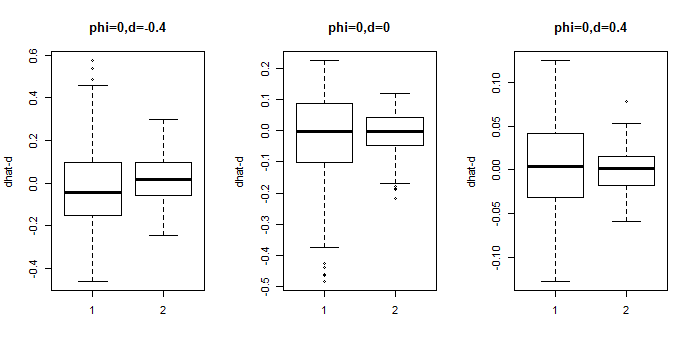
\includegraphics[width=14.5cm]{Rplot01}
\caption{the left side is n=1024 and the right side is n=4096}
\end{figure}

\begin{figure}[!htb]
\centering
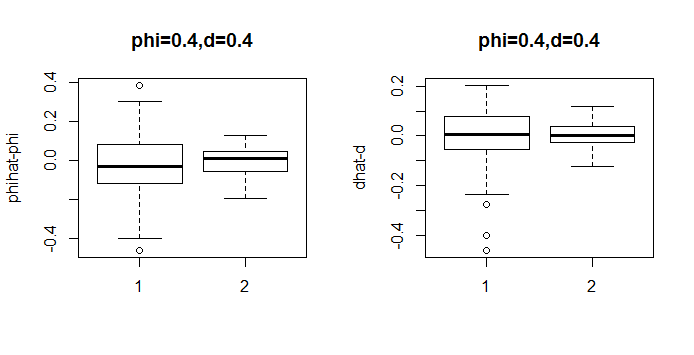
\includegraphics[width=14.5cm]{Rplot02}
\caption{the left side is n=1024 and the right side is n=4096}
\end{figure}
Some conclusions from Table 3 and Boxplots:
\begin{itemize}
\item {no significant bias observed }
\item {the standard deviation decreases when the sample size becomes large}
\item {the performance of spectral maximum likelihood is not so good since relatively large standard deviation and existence of outliers }
\item {the AR coefficient are hard to estimate using Nelder–Mead method in two ways: 1. it mostly gives unreasonable result even we set start points to be the true value. 2. when MA coefficients are estimated, the computational time becomes surperingly expensive, this is why we didn't conduct simulations for $q>0$ in ARFIMA(p,d,q)}
\end{itemize}

We estimate coefficient of log sqared BUCH data, Nelder–Mead method yields $\sigma_\eta^2=0.780,\, \sigma_\epsilon^2=4.403,\,\phi= 0.137,\,d=0.417$, MCMC method yields $ \sigma_\eta^2=0.537,\, \sigma_\epsilon^2=5.00,\,\phi= 0.135,\,d=0.434 $ 

In Figure 7, we use the estimated coefficients to run simulation for 100 replications and plot the mean acf with the acf of data. We can see the LMSV model with estimated data fits well, it clearly shows the hyperbolical decay of acf.
\begin{figure}[!htb]
\centering
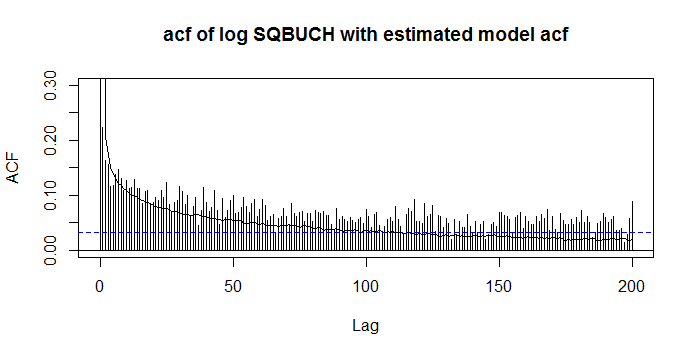
\includegraphics[width=14.5cm]{Rplot3}
\caption{}
\end{figure}


\section{Conclusion}
In GARCH, EGARCH, IGARCH model, the variance depends on past variances and  in some books(Ruey S.Tsay(2005))\cite{tsay2005analysis} it is called observation driven. While LMSV model introduced in this paper is not a observation driven model. It is driven by a unobserved stochastic process. An additional random variable $\eta$ is introduced to provide more information. The LMSV model can be simplied to an ARFIMA(p,d,q) model plus a noise, which has many well understood properties.

The paper introduces two method of testing for long memory. In the simulation study we see long memory and short memory are distinguishable. 

Spectral MLE estimator is consistent and performs well on large sample, the emprical experience shows the LMSV model with Spectral MLE estimators fit BUCH data well.

Further, some recent papers report this model and spectral MLE suffers from level shifts and outliers in both full-parametric and semiparametric estimate. See, i.e Diebold and Inoue (2001)\cite{diebold2001long}, Granger and Hyung (2004)\cite{granger2004occasional},
Mikosch and Starica (2004)\cite{mikosch2004nonstationarities}, Perron and Qu (2010)\cite{shumway2000time} and McCloskey, Adam and Perron, Pierre(2013)\cite{mccloskey2013memory}(we didn't dig into these paper, just read the abstracts.).

\renewcommand\refname{Reference}
\bibliographystyle{plain}
\bibliography{writeup} 
We also refers some unpublished instruction or slides. see(\url{https://github.com/lunge111/STA237PROJECT})
\end{document}


